\documentclass[tikz]{standalone}
\usetikzlibrary{mindmap}
\begin{document}
    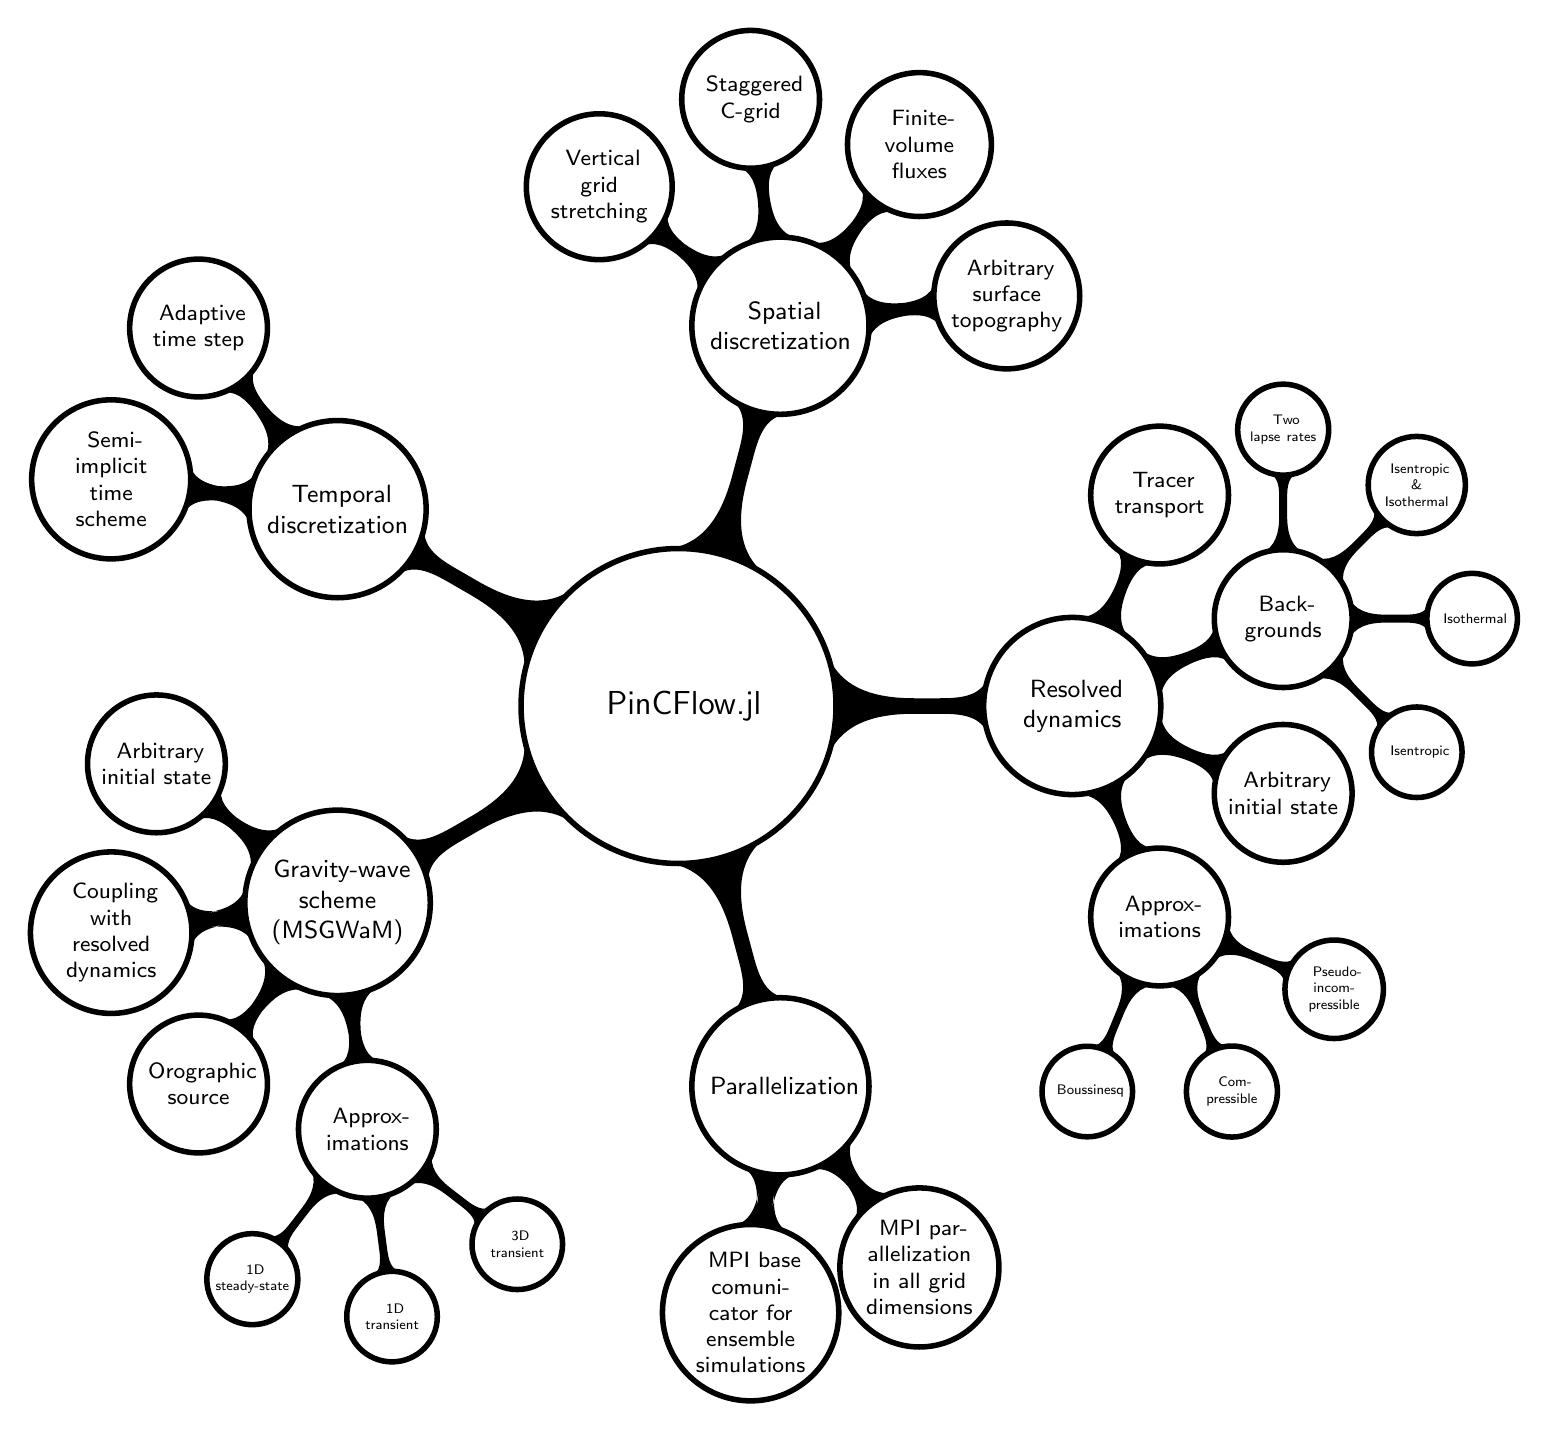
\begin{tikzpicture}[mindmap, grow cyclic, line width = 2pt, execute at begin node = ~\textsf, every node/.style = {concept, fill = white}, level 1/.append style = {sibling angle = 75}, level 2/.append style = {sibling angle = 45}, level 3/.append style = {sibling angle = 45}]
        \node {PinCFlow.jl}
            child {node {Gravity-wave scheme (MSGWaM)}
                child {node {Arbitrary initial state}}
                child {node {Coupling with resolved dynamics}}
                child {node {Orographic source}}
                child {node {Approximations}
                    child {node {1D steady-state}}
                    child {node {1D transient}}
                    child {node {3D transient}}}}
            child {node {Parallelization}
                child {node {MPI base comunicator for ensemble simulations}}
                child {node {MPI parallelization in all grid dimensions}}}
            child {node {Resolved dynamics}
                child {node {Approximations}
                    child {node {Boussinesq}}
                    child {node {Compressible}}
                    child {node {Pseudo-incom-pressible}}}
                child {node {Arbitrary initial state}}
                child {node {Backgrounds}
                    child {node {Isentropic}}
                    child {node {Isothermal}}
                    child {node {Isentropic \& Isothermal}}
                    child {node {Two lapse rates}}}
                child {node {Tracer transport}}}
            child {node {Spatial discretization}
                child {node {Arbitrary surface topography}}
                child {node {Finite-volume fluxes}}
                child {node {Staggered C-grid}}
                child {node {Vertical grid stretching}}}
            child {node {Temporal discretization}
                child {node {Adaptive time step}}
                child {node {Semi-implicit time scheme}}};
    \end{tikzpicture}
\end{document}
